\section{Resultados}

\subsection{Human Phenotipe Ontology}

\hfill

Tras realizar una búsqueda del fenotipo a investigar, \textit{Dyscalculia}, vemos que se encuentra clasificado como \href{https://hpo.jax.org/app/browse/term/HP:0002442}{HP:0002442} con un total de 13 fenotipos de otras enfermedades asociadas y un total de 24 genes asociados a esta en HPO.

Añadir tabla de HPO

\subsection{String}

\hfill

Gracias a las anotaciones en HPO, podemos obtener los genes asociados del fenotipo, y con ello procedemos a la búsqueda de más información a cerca de estos utilizando \href{https://string-db.org}{STRING}, una base de datos biológica y un recurso web de interacciones entre proteínas.

\begin{figure}[h]
	\centering
	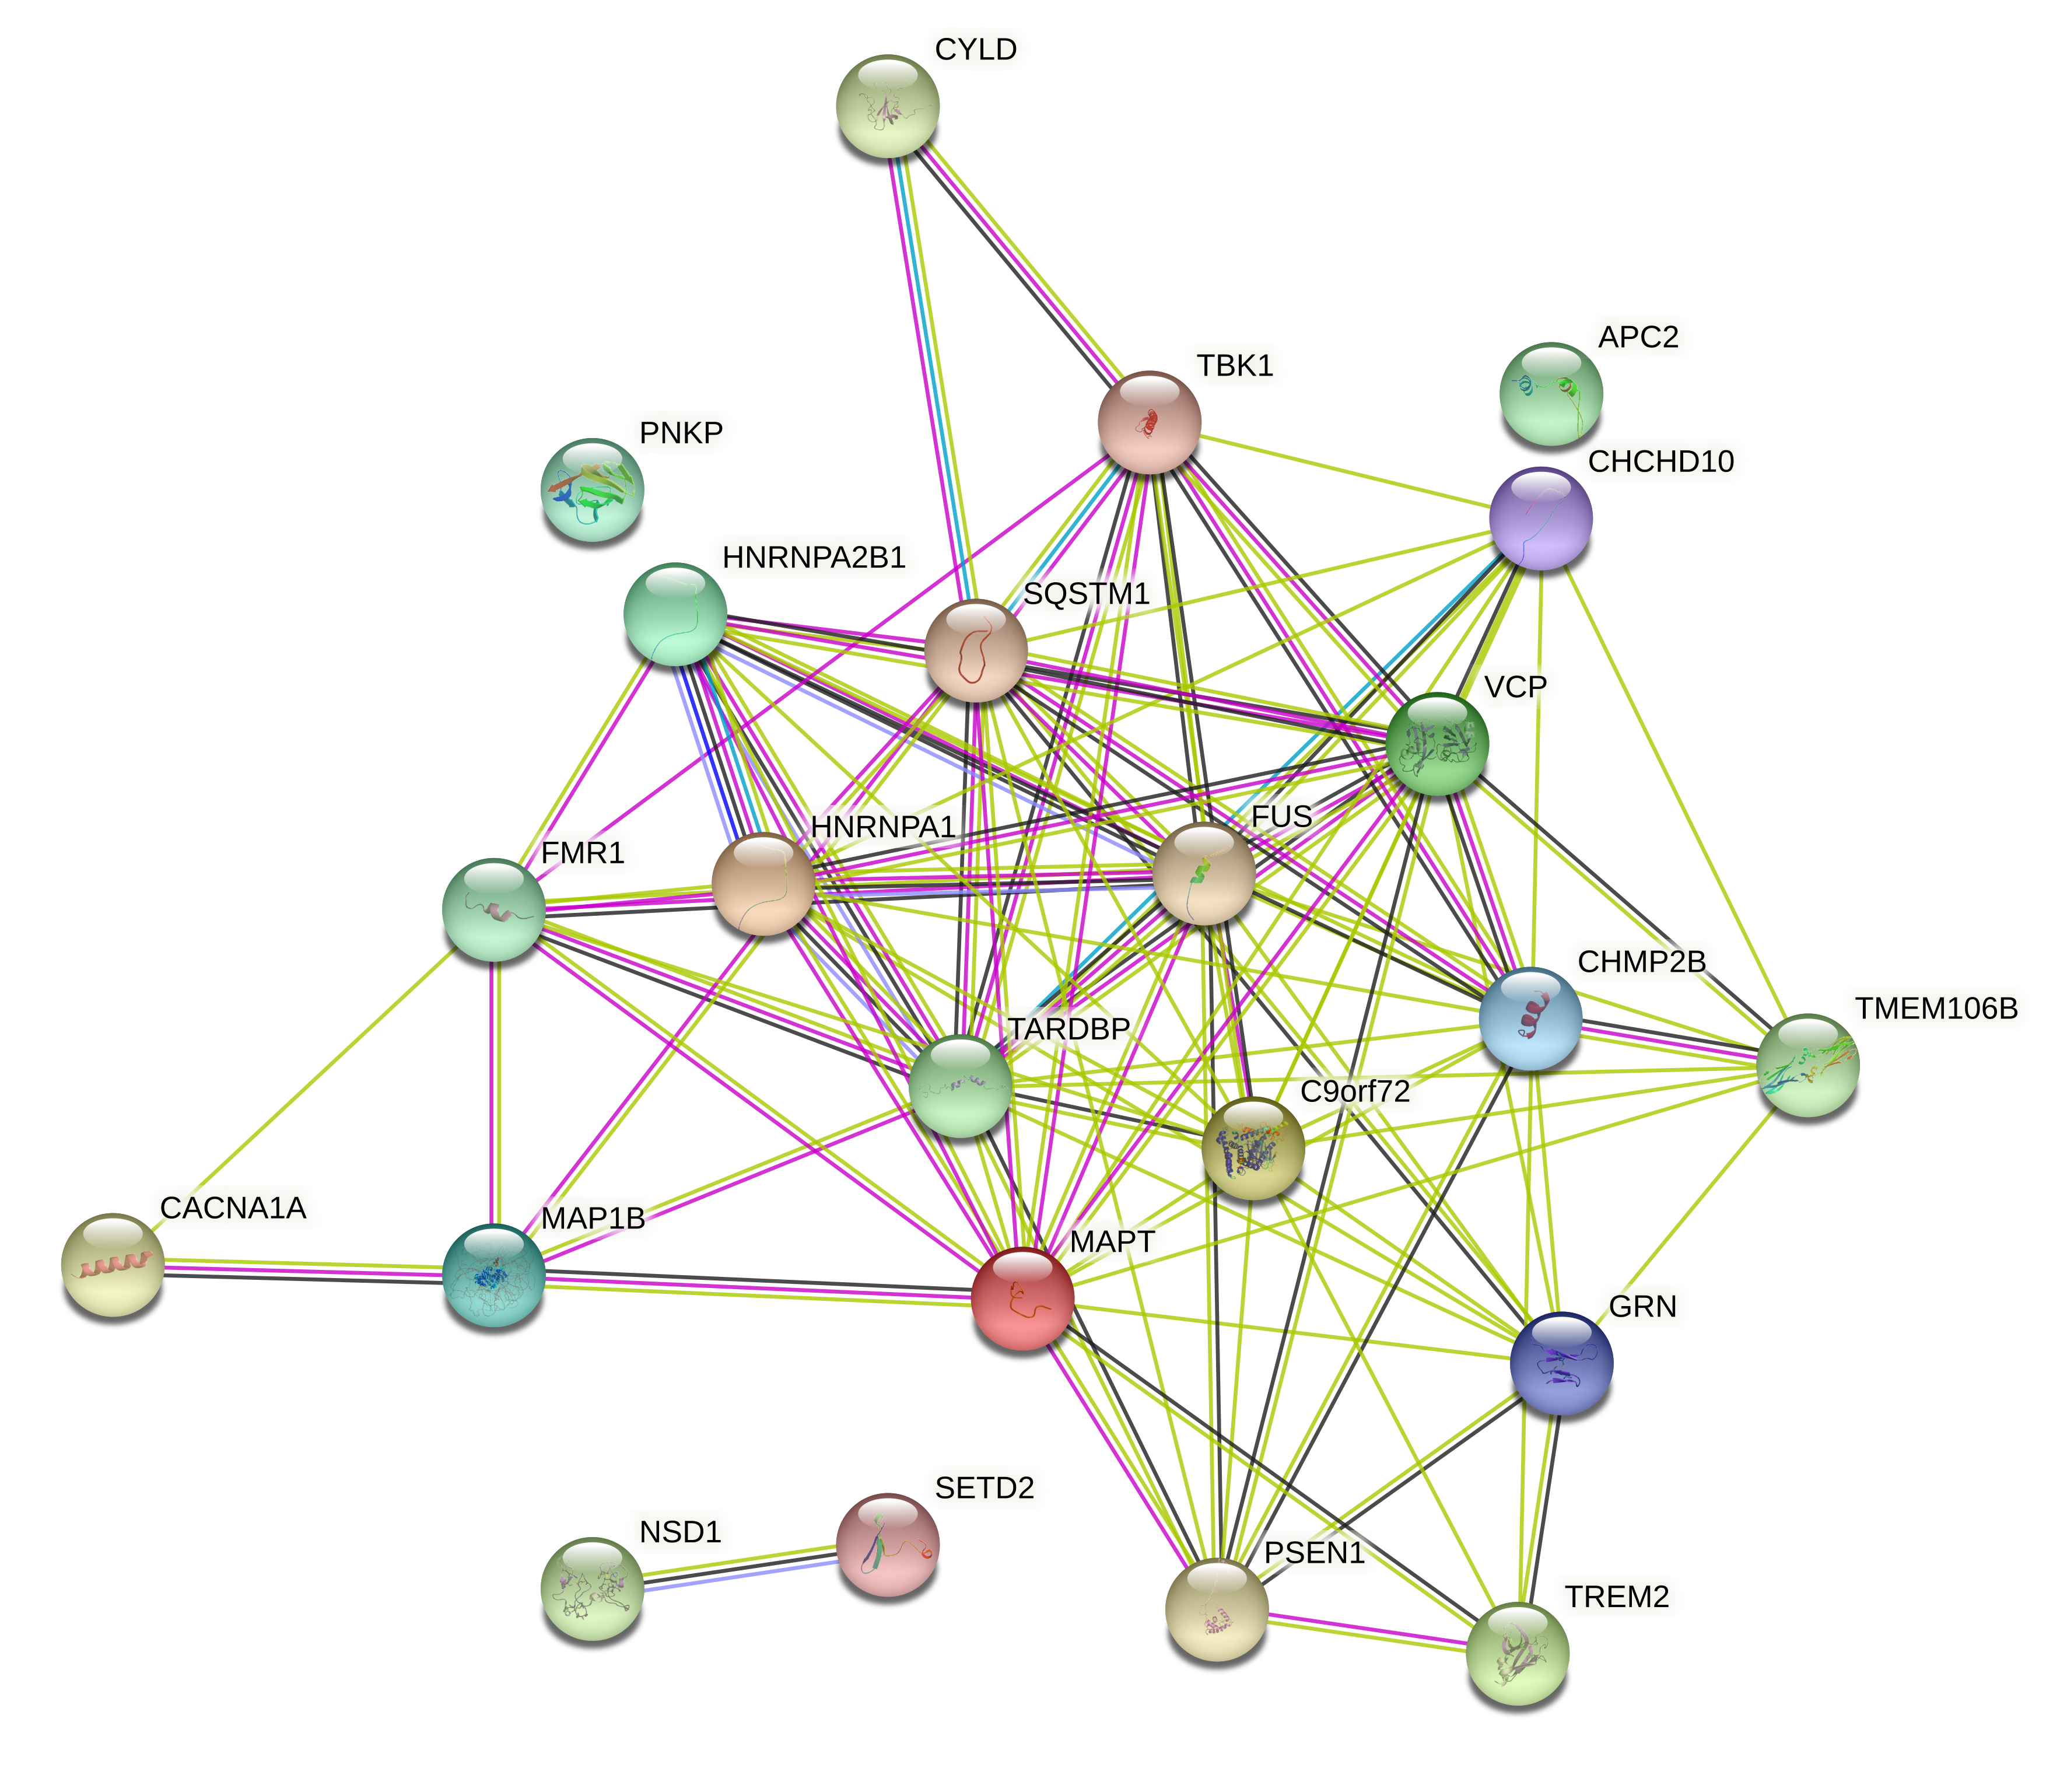
\includegraphics[width=0.90\textwidth]{figures/Gene_Relationship.png}
	\caption{Interacciones proteína-proteína a raíz de los genes relacionados. }
	\label{fig:string1}
\end{figure}


\hfill
